\section{Arquitectura capa de negocio}
{Esta capa, es la capa de arquitectura del proyecto orientada al negocio, aquí se plasma el enfoque organizacional, las reglas que regirán el negocio y las entidades que representan el sistema, permitiendo obtener de forma optima los roles y actores que aquí se desempeñan.}

	\subsection{Punto de vista de organización}
	{ El punto de vista organizacional esta enfocado a la estructura interna de la empresa, departamento o entidad organizacional, este refleja de forma jerárquica el nivel de los actores y roles que aquí interactúan \cite{archimate}.\\
		
		\textbf{Modelo}\\
		\begin{figure}[H]
			\centering
			\includegraphics[width=0.8\linewidth]{development/organizacion.png}
			\caption{Metamodelo de Organización}
		\end{figure}
	
		\textbf{Caso}\\
		
		\begin{figure}[H]
			\centering
			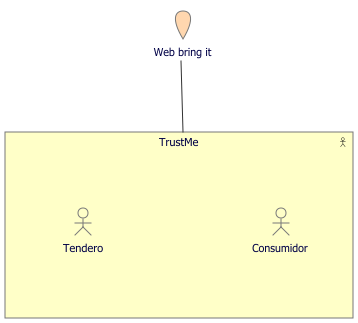
\includegraphics[width=0.8\linewidth]{development/negocio.pdf}
			\caption{Organización}
		\end{figure}
	}
	
	\subsection{Punto de vista de cooperación de actor}
	{ 
		
		\textbf{Modelo}\\
		\begin{figure}[H]
			\centering
			\includegraphics[width=0.8\linewidth]{development/cooperacionactor.png}
			\caption{Metamodelo de cooperación de actor}
		\end{figure}
		
		\textbf{Caso}\\
		
		\begin{figure}[H]
			\centering
			\includegraphics[width=0.8\linewidth]{development/cooperacionactor.pdf}
			\caption{Cooperación de actor}
		\end{figure}
	}
	
	\subsection{Punto de vista de función de negocio}
	{ 
		
		\textbf{Modelo}\\
		\begin{figure}[H]
			\centering
			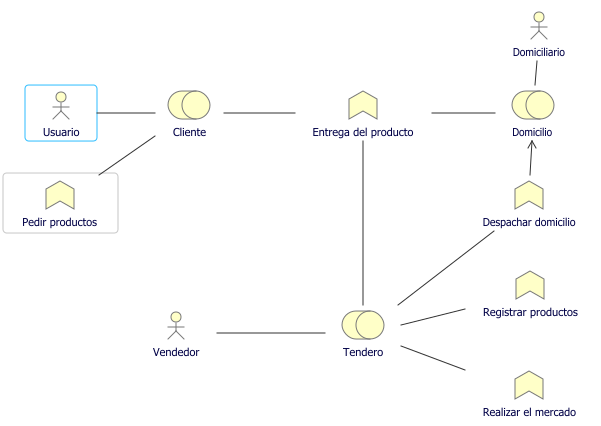
\includegraphics[width=0.8\linewidth]{development/funcion.png}
			\caption{Metamodelo de función de negocio}
		\end{figure}
		
		\textbf{Caso}\\
		
		\begin{figure}[H]
			\centering
			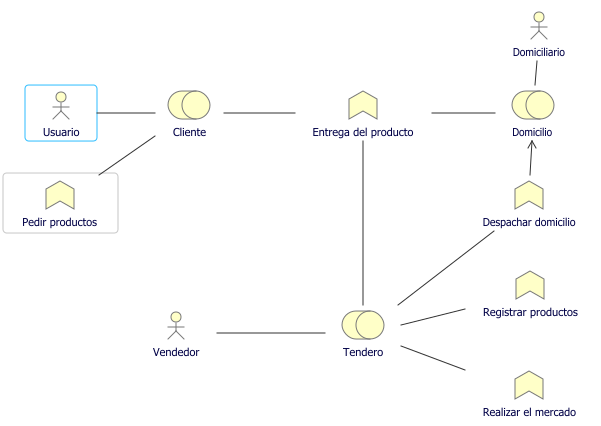
\includegraphics[width=0.8\linewidth]{development/funcion.pdf}
			\caption{Función de negocio}
		\end{figure}
	}
	
	\subsection{Punto de vista de proceso de negocio}
	{ 
		
		\textbf{Modelo}\\
		\begin{figure}[H]
			\centering
			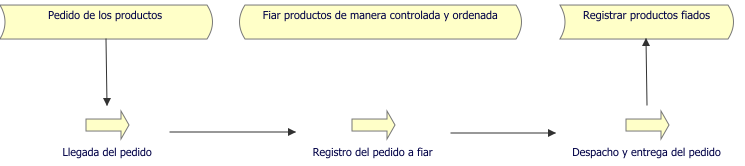
\includegraphics[width=0.8\linewidth]{development/proceso.png}
			\caption{Metamodelo de proceso de negocio}
		\end{figure}
		
		\textbf{Caso}\\
		
		\begin{figure}[H]
			\centering
			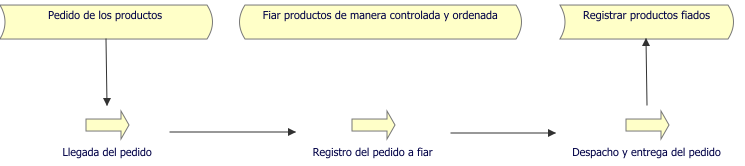
\includegraphics[width=0.8\linewidth]{development/proceso.pdf}
			\caption{Proceso de negocio}
		\end{figure}
	}
	
	\subsection{Cooperación de proceso de negocio}
	{ 
		
		\textbf{Modelo}\\
		\begin{figure}[H]
			\centering
			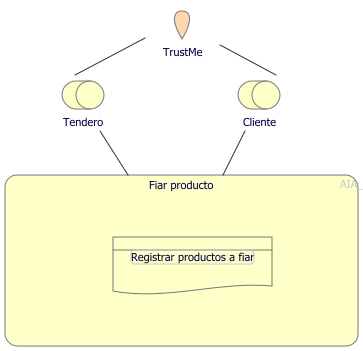
\includegraphics[width=0.8\linewidth]{development/cooperacionproceso.png}
			\caption{Metamodelo de cooperación de proceso de negocio}
		\end{figure}
		
		\textbf{Caso}\\
		
		
		\begin{figure}[H]
			\centering
			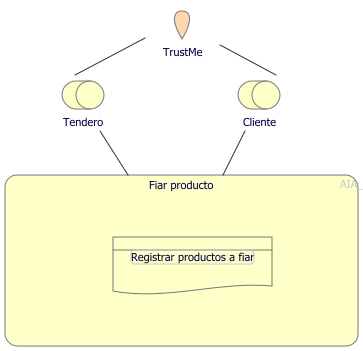
\includegraphics[width=0.8\linewidth]{development/cooperacionproceso.pdf}
			\caption{Cooperación de proceso de negocio}
		\end{figure}
	}
	
	\subsection{Punto de vista de producto}
	{
		
		\textbf{Modelo}\\
		\begin{figure}[H]
			\centering
			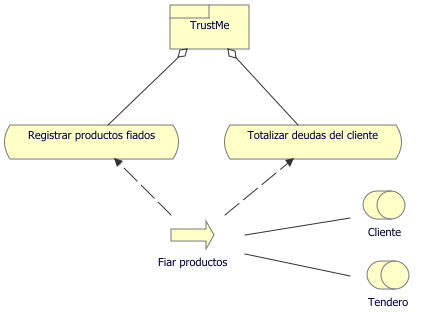
\includegraphics[width=0.8\linewidth]{development/producto.png}
			\caption{Metamodelo de producto}
		\end{figure}
		
		\textbf{Caso}\\
	
		
		\begin{figure}[H]
			\centering
			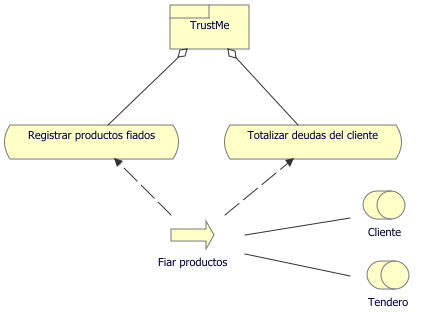
\includegraphics[width=0.8\linewidth]{development/producto.pdf}
			\caption{Producto}
		\end{figure}
	}